% Copyright (c) 2014,2016 Casper Ti. Vector
% Public domain.

\chapter{相关工作}  \label{chap:related}
\section{分布式数据库HBase}
HBase是Google BigTable\supercite{bigtable}的开源实现 ,是Hadoop 生态系统中一个列式NoSQL数据库,搭建在HDFS(Hadoop分布式文件系统)之上。HBase由于其优异的可扩展性和稳定性,在产业界得到了广泛应用。
下面分别介绍HBase的数据模型、操作接口、系统架构、存储实现以及HBase与同类系统的对比。

\subsection{HBase数据模型}
在HBase中,数据首先以表为单位进行组织。数据表以行为单位组织,每行由一个键值唯一标识,称为行键(row key)。一行中可以包含任意列的数据,每列对应的数据可分为多个版本(对应多个时间戳)。每个版本的数据是最小粒度的数据单元,称为一个单元格(cell)。因此一个单元格由行键、列名、版本号(时间戳)和值(value)组成。
在HBase中,各列按列族(column family)进行组织,因此列名实际由列族名和列修饰符(column qualifier)组成。区别于传统关系模型,列族里的列修饰符可以随时添加,不需要事先定义。即在插入数据时,可以指定任意的列修饰符。行键是每个表必须要有的一列,且只能是唯一的一列,不属于任何列族。图\ref{fig:hbase_table}是HBase中一张数据表的示例。

\begin{figure}[htbp]
\centering
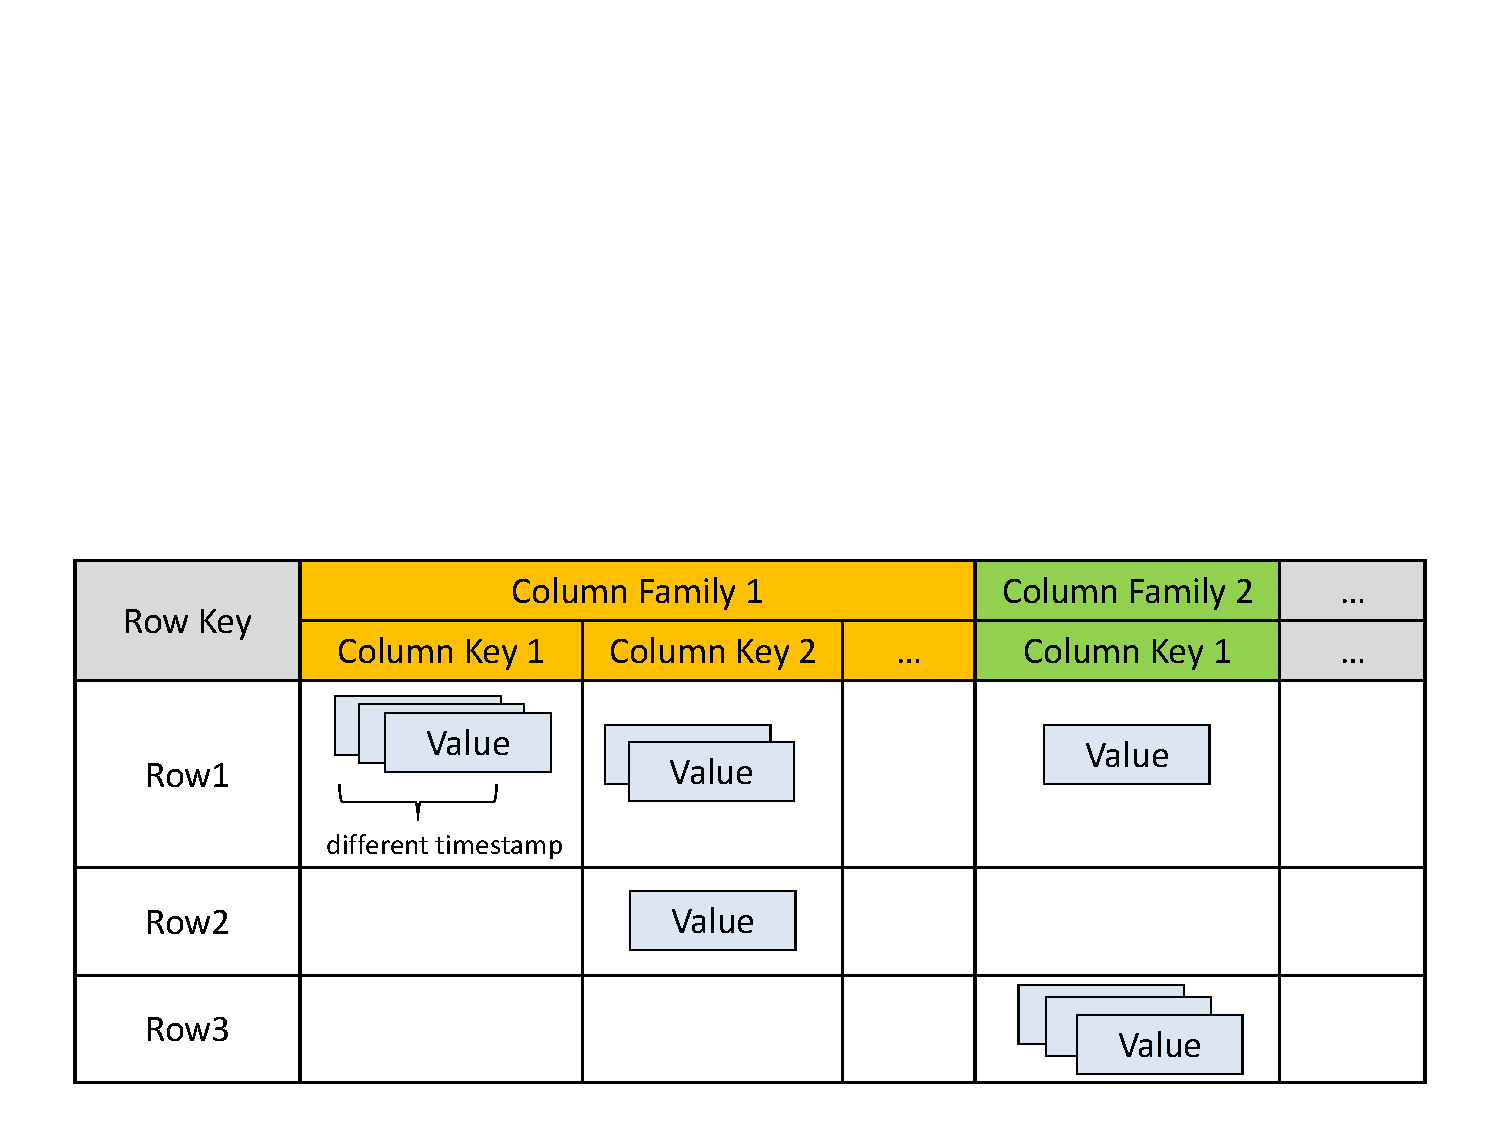
\includegraphics[width=120mm]{fig/HBase_table_example.pdf}
\caption{HBase数据表示例}
\label{fig:hbase_table}
\end{figure}

HBase也被认为是一个键值存储(Key-Value Store),相当于数据结构Map的存储。这是因为每个单元格实际存储的是Value部分,而Key部分就是由行键、列族名、列修饰符和时间戳合并构成。由于列修饰符是不需要事先定义的,因此整个Key部分是可以随意指定的,从而可以将HBase归类为键值存储。图\ref{fig:hbase_cell}是一个Cell的数据组成以及如何表示为键值对的示例。单元格也确实是HBase的存储实现中的最小单元,因此将HBase归类为键值存储。

\begin{figure}[htbp]
\centering
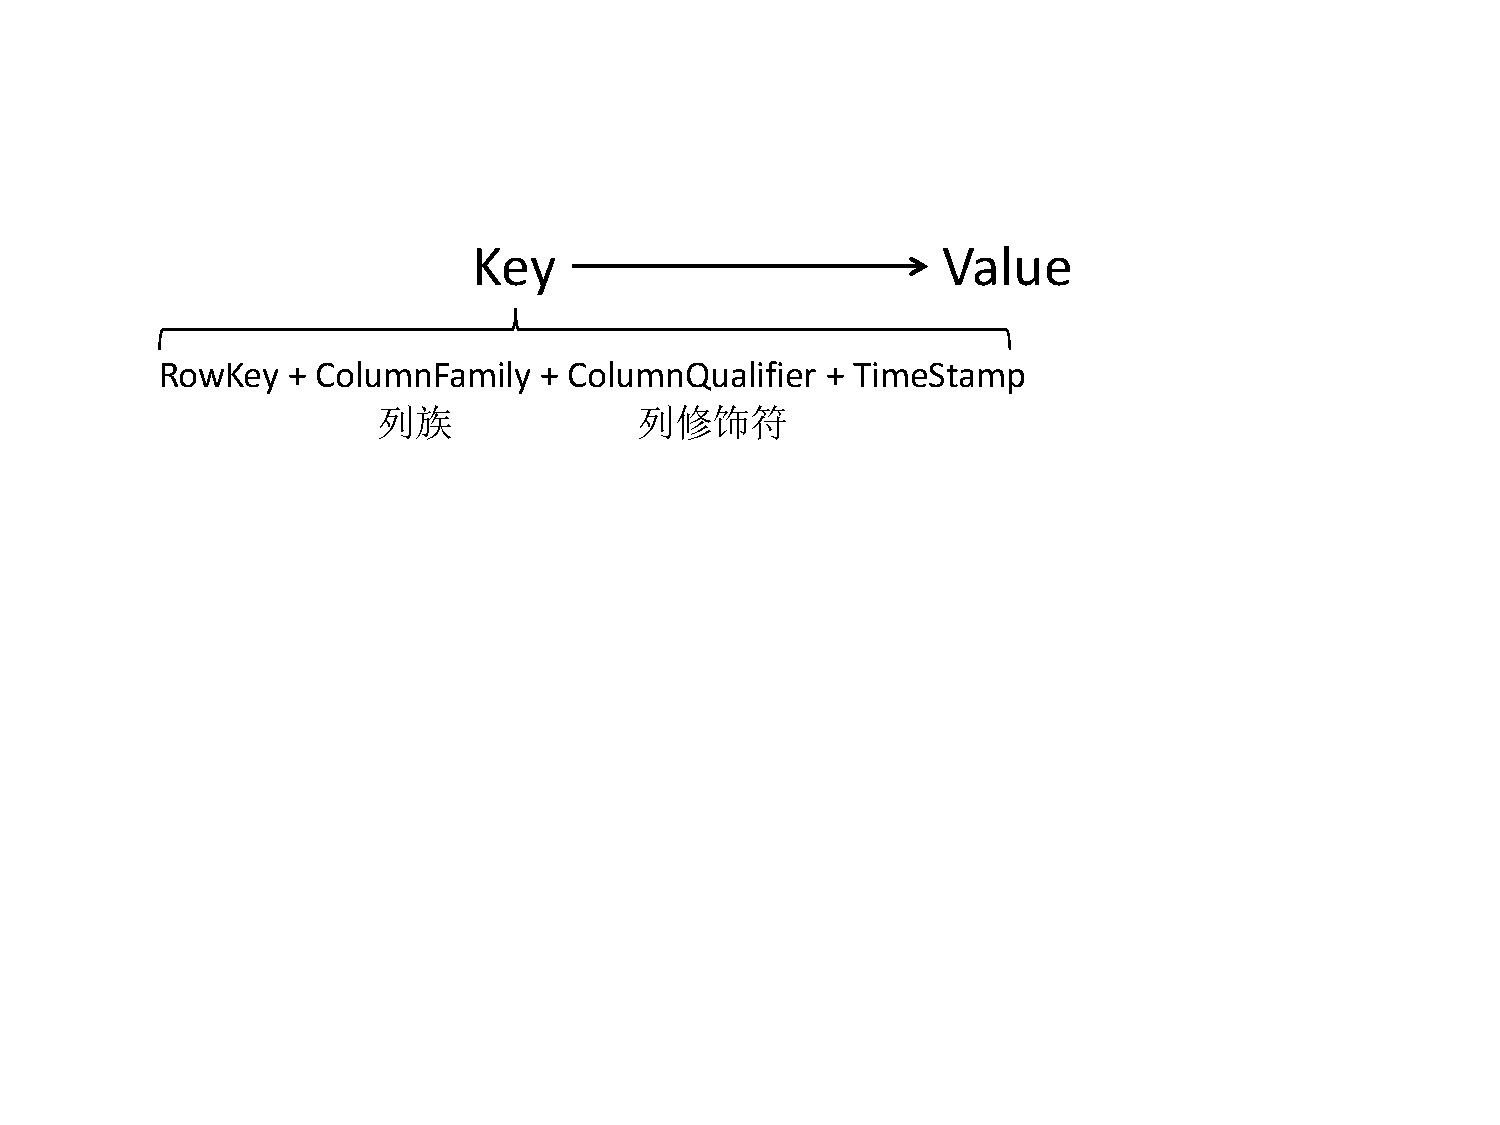
\includegraphics[width=120mm]{fig/HBase_key_value.pdf}
\caption{HBase中Cell单元的Key、Value成分}
\label{fig:hbase_cell}
\end{figure}

\subsection{HBase操作接口}
HBase提供了一个交互式的shell作为操作接口,同时也提供原生的Java接口,另外还提供了thrift API,支持C++、Python、Ruby、Perl、PHP等语言。下面以HBase shell为例叙述HBase的操作接口。

HBase建表时需要指定表中的所有列族,在建表之后还可以增加或删除列族,如下所示:
\begin{verbatim}
HBase Shell > create 'table1', 'cf1', 'cf2'
HBase Shell > alter 'table1', 'delete' => 'cf1'
HBase Shell > alter 'table1', 'cf3'
\end{verbatim}

HBase提供Put、Get、Scan、Delete接口进行数据的增删查改。Put接口给某一行中插入一个单元格。Delete接口跟Put接口相反,用来删除一个单元格的数据 。Get接口跟Scan接口用来读取数据。其中Get接口能读取的范围不超过一行,即Get接口可以读取一个单元格,也可以读取一行中所有的单元格,但读取的对象都只能在同一行中。Scan接口则用来读取连续的多行数据


Get接口能读取某一单元格的数据,也能读取某一行所有单元格的数据。
,能够具体操作一行中的给定列。另外,HBase提供给定行键范围的Scan接口,可以快速地获得连续几行的数据。Scan接口也可指定特定的列或附加Filter来过滤无关数据。

\begin{verbatim}
HBase Shell > create 'table1', 'cf1', 'cf2'
HBase Shell > put 'table1', 'row1', 'cf:a', 'value1'
HBase Shell > put 'table1', 'row2', 'cf:b', 'value2'
HBase Shell > put 'table1', 'row1', 'cf:b', 'value3', timestamp1

\end{verbatim}

在本节也可以看到,HBase并没有提供类型关系数据库的SQL接口,这是所有NoSQL数据库的一个特点,都是根据自己的数据模型因地制宜地提供对应的接口。

% ACID的支持情况是否要说?

\begin{figure}[htbp]
\centering
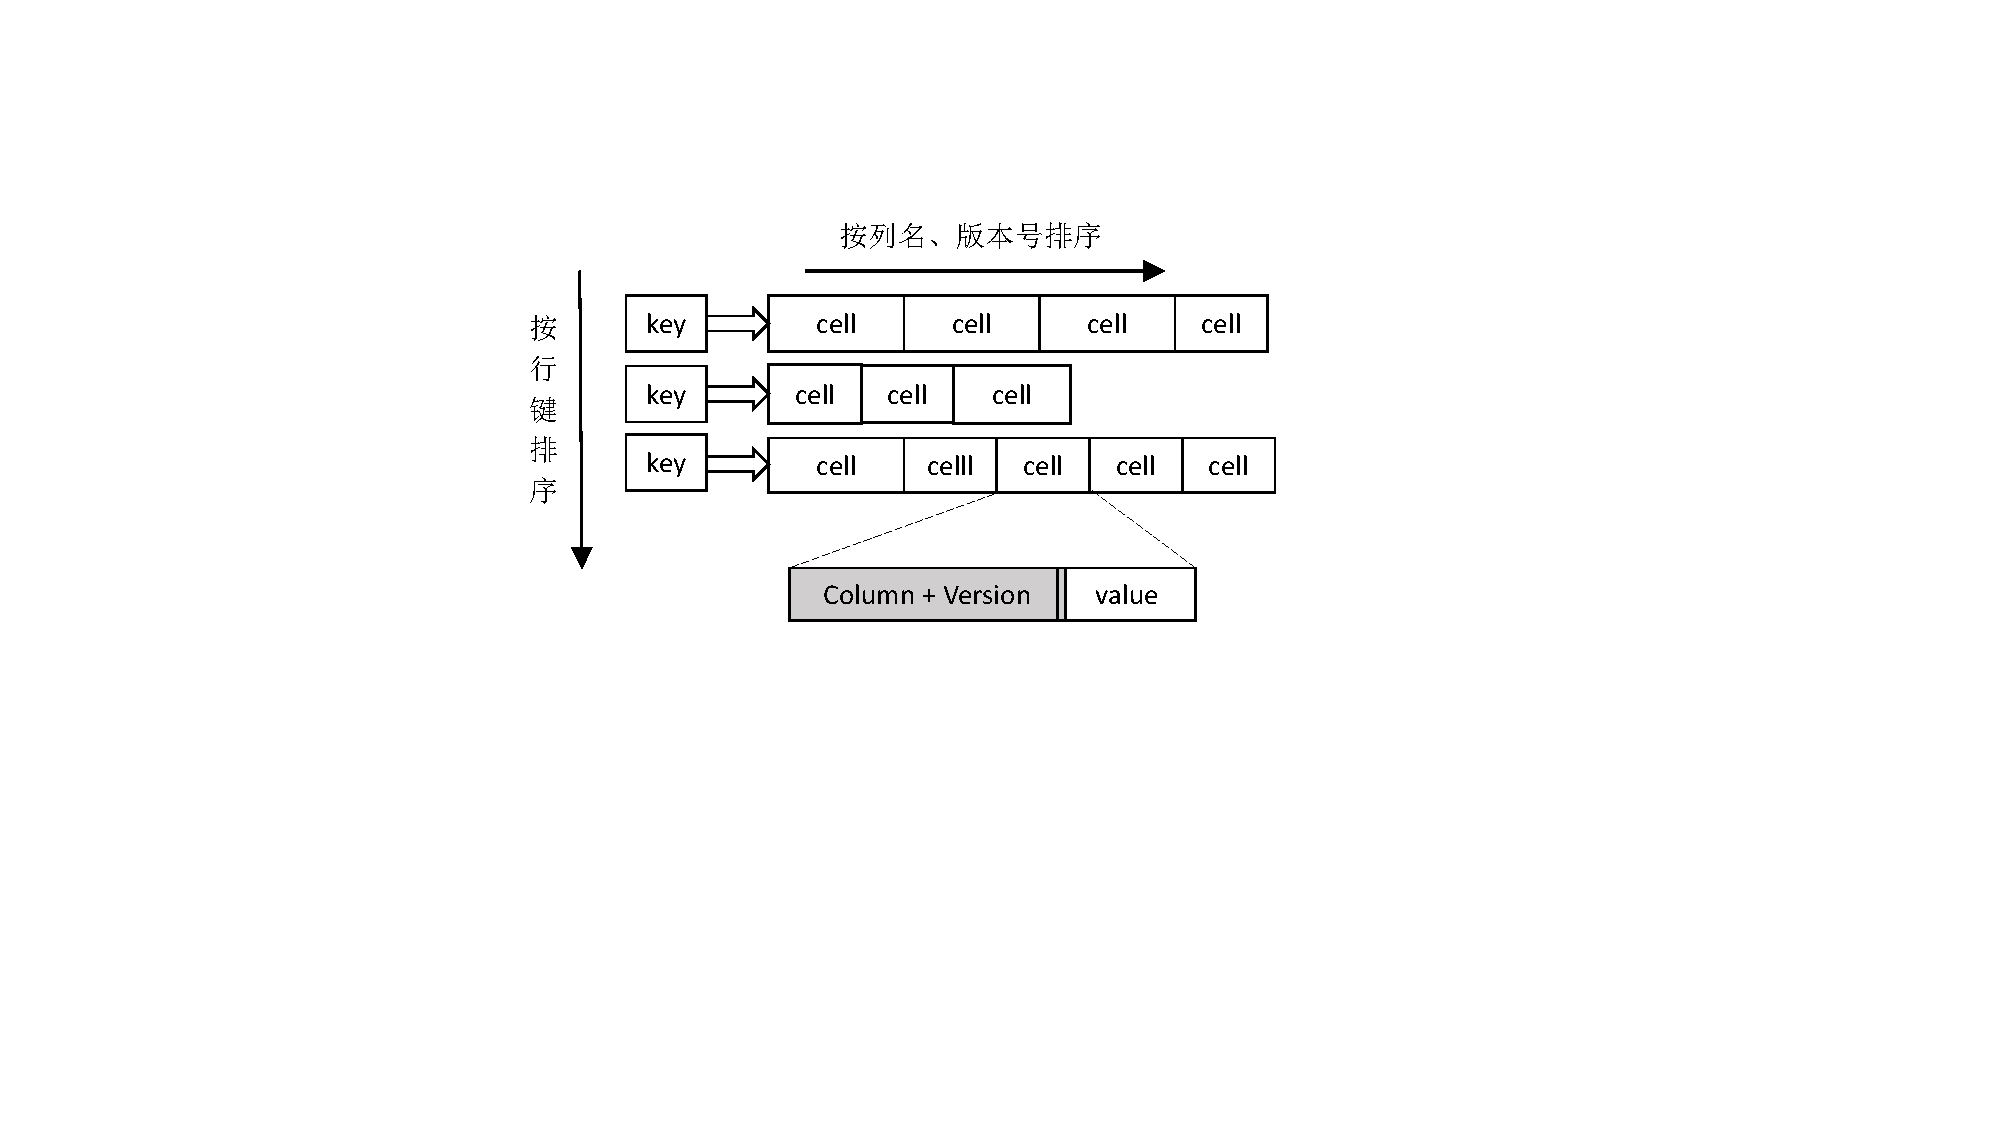
\includegraphics[width=100mm]{fig/big_table.pdf}
\caption{BigTable模型示例}
\label{fig:big_table}
\end{figure}

BigTable是Google在2008年提出的一个处理海量数据的NoSQL数据库。图\ref{fig:big_table}是BigTable的模型示例。在BigTable的模型中,数据表以行为单位组织,每行由一个键值唯一标识,称为行键(rowkey)。一行中可以包含任意数目的单元格(cell),每个单元格由列名、版本号(时间戳)和值(value)组成。BigTable中的行是以行键排序的,每一行中的单元格又是以列名和版本号进行排序,这使得其与关系数据库一样能快速定位到目标单元格。区别于传统关系模型,BigTable中的列名不需要事先定义,因为其底层实际为一个Key-Value 存储,就如数据结构Map不需要事先定义所有key。每个列名从属于一个列族,只有列族需要在定义表结构时给出。


\subsection{HBase系统架构}
\subsection{HBase存储实现}


\subsection{HBase与同类系统对比}

\section{图数据库Titan}
图数据库是以图的形式来表示和管理数据的数据库\supercite{graph_models_survey},与传统的关系型数据库相比,图数据库在图结构相关的查询上有更优异的性能,如多跳邻域查询、路径查询、局部聚集系数计算等。
Titan是一个基于Blueprints 接口设计的开源图数据库,其实现了一个可插拔的存储接口,可以部署在BerkerlyDB 、HBase或Cassandra之上。相比于著名的图数据库Neo4j,Titan是完全开源免费的,其受关注度正在与日俱增。而且由于Hadoop生态系统在产业界的广泛应用,在HBase上搭建Titan,即使用Titan on HBase应对图处理需求是较为常见的选择。

\subsection{Titan存储实现}
在图数据库Titan中,基于BigTable模型,数据在HBase中以邻接表的形式存储,如图\ref{fig:adj_list}所示。

\begin{figure}[htbp]
\centering
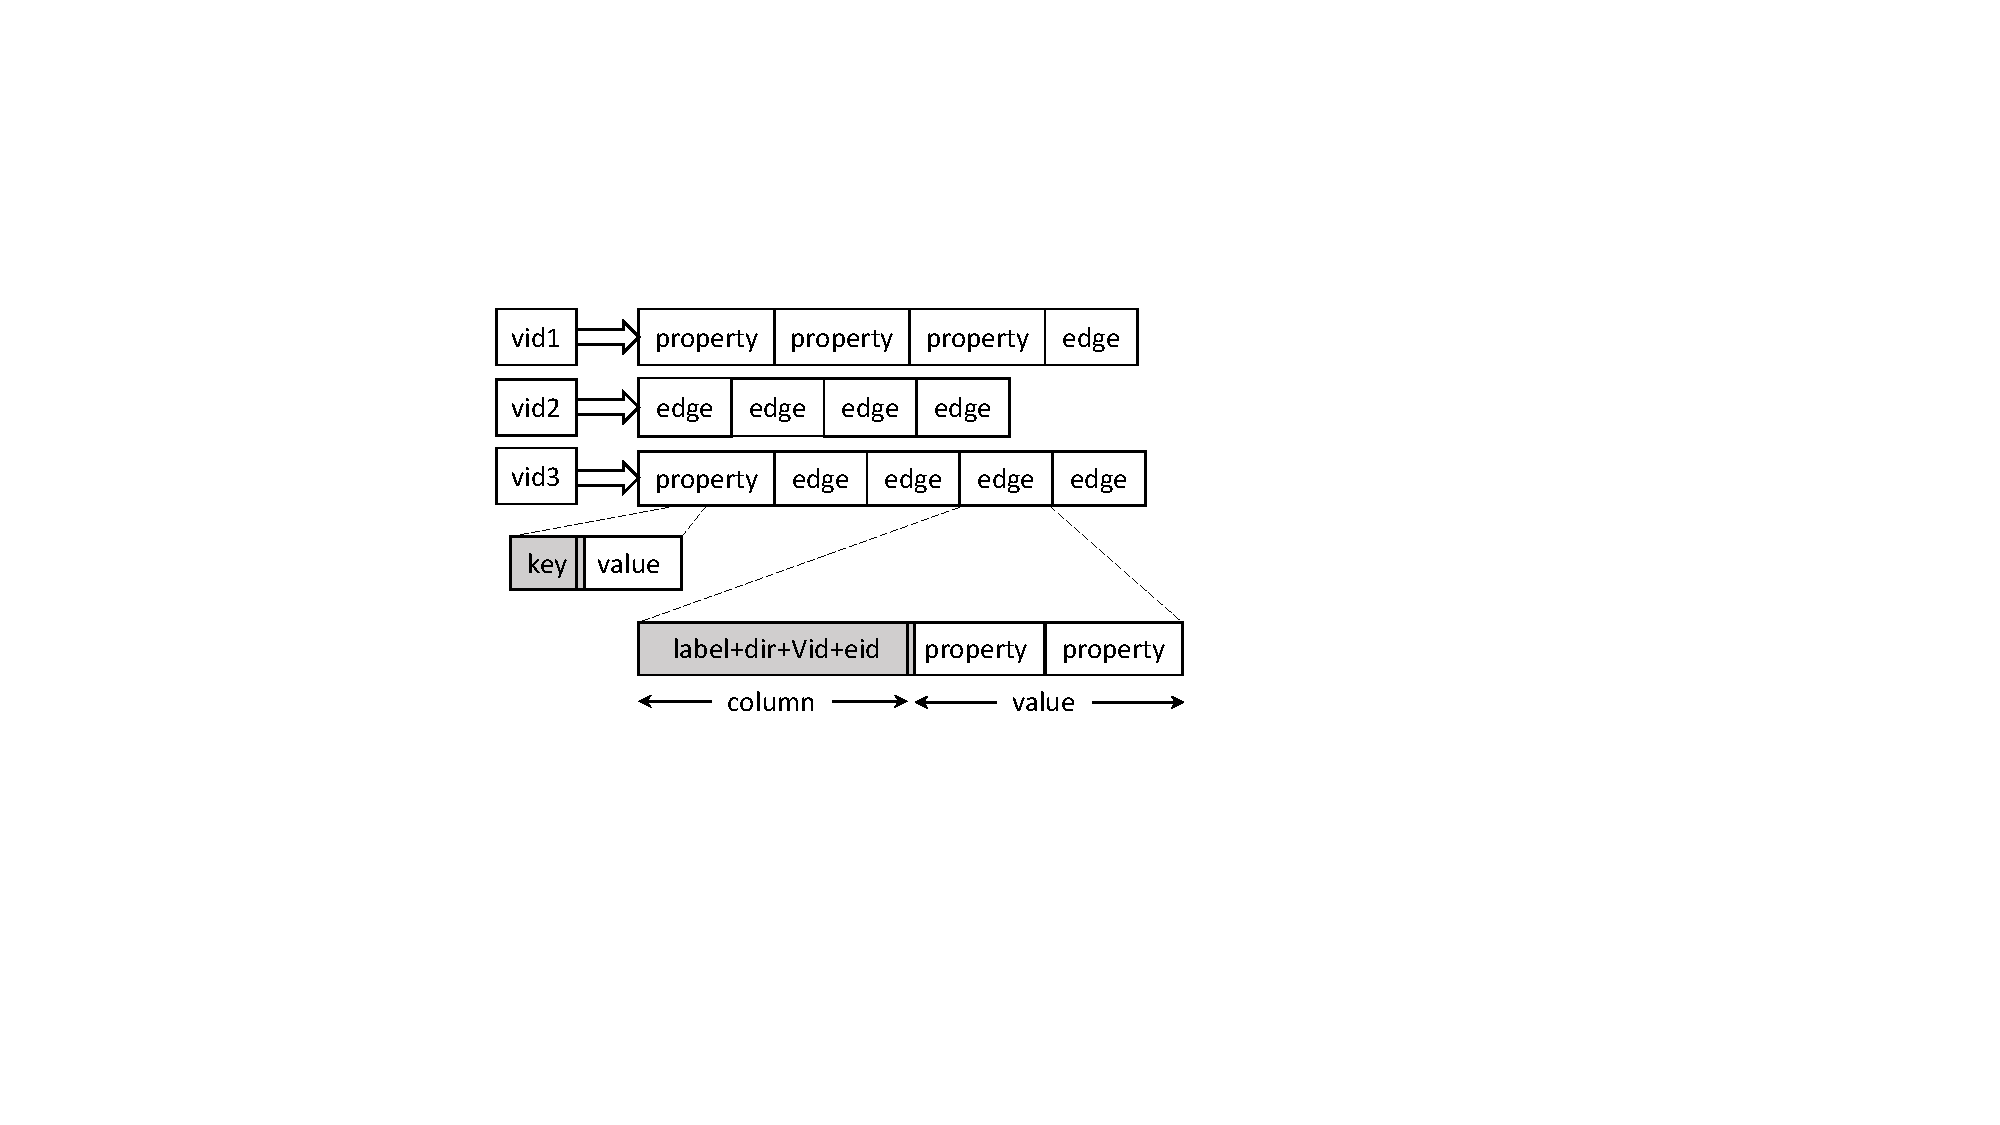
\includegraphics[width=100mm]{fig/adj_list.pdf}
\caption{Titan内部的BigTable实现}
\label{fig:adj_list}
\end{figure}

Titan为每个点分配了一个全局唯一的id,每个点占BigTable中的一行,行键就是点的id。每行存储了该点相关的属性和边,它们各占一个单元格。Titan在BigTable模型中设置最大版本数为1,从而使每行中的列名与单元格一一对应,根据行键和列名可以快速定位到目标单元格,实现对边和属性内容的快速检索。

在Titan中,每个属性是一个key-value对。点的属性存储在该点所在的行,每个属性占一个单元格,并以属性名key作为列名,这使得每个点的属性查询可以非常高效。

每个点所在的行还存储了邻接的所有边数据,每条边占一个单元格。一条边的信息包含了邻接点、类别(label)、方向、边的唯一id,以及边上的各属性。单元格的值用来存储边上的所有属性,列名则存储边上除属性外的其它信息。在BigTable模型中,同一行的单元格按列名排序。为了方便检索,每条边所在的单元格依次以label、方向、邻接点id以及边id拼接成为列名,即
\begin{center}
  列名 = 边label + 方向 + adjVid + eid
\end{center}
这种列名设计使得一个点的所有边先按label排序,再按方向、邻接点id、边id等排序。其优点是当要检索该点指定label的所有边时,只需要扫描邻接表的一部分。图4是一个更详细的示例。

\subsection{图数据库Titan的局限性}
当图中的重边数量巨大时,Titan的邻接表列数也急剧变大,这会对邻域中点和边的检索带来严重影响。

\begin{figure}[htbp]
\centering
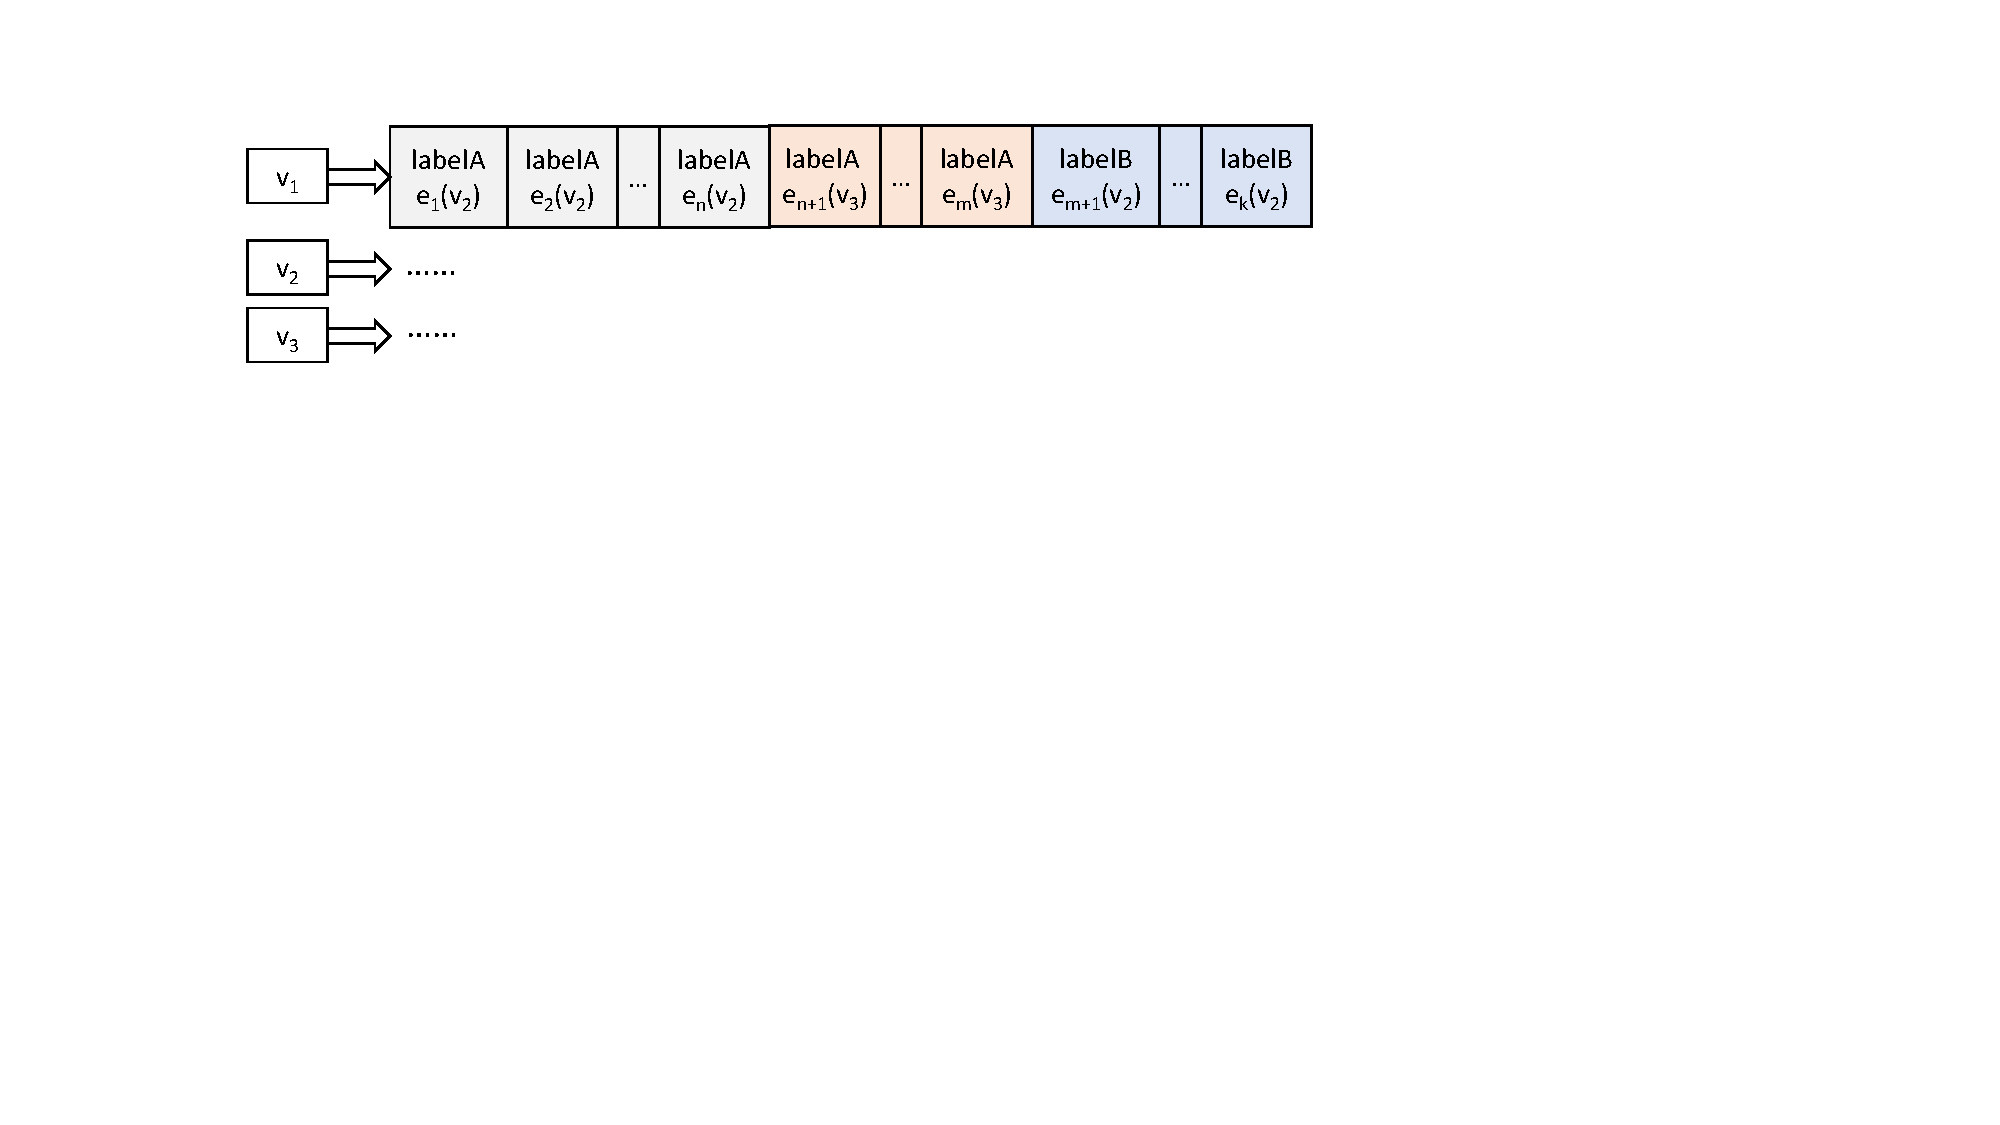
\includegraphics[width=150mm]{fig/original_list.pdf}
\caption{当属性图富含重边时,Titan在HBase中的数据表是一张扁平而宽的表}
\label{fig:orginal_list}
\end{figure}

图\ref{fig:orginal_list}展示了一个富含重边的场景,为方便展示省略了边的方向。v1只有v2和v3两个邻接点,其中与v2有两种label的边,与v3有一种label的边。虽然邻接的点数不多,但v1与邻接点都有数量巨大的重边。由于邻接表存储的是每条边的信息,当要查询v1的所有邻接点集(即v1、v2)时,不得不遍历一次v1的所有边,即遍历整个邻接表。当重边数量巨大时,这是大量的无谓开销。

为了规避上述情形,我们可以换一种列名设计来优化邻域点集查询,比如让邻接表先按邻接点id排序,令
\begin{center}
  列名 = adjVid + 边label + 方向 + eid
\end{center}
这样当发现一个邻接点时,可以跳过相同邻接点的所有边,不用再遍历整个邻接表。然而,面对label相关的查询时又会面临同样的问题,比如查询该点总共有几种label的边,仍需要遍历该点的整个邻接表。因此,改变邻接表的列名设计并不能解决问题,本质原因是邻接表存储了所有的边集。

另一方面,Titan为加快数据访问设计了缓存,存储最近访问的点及其邻接表内容。如果图中各点的重边都很多,则缓存空间被大量的重边占满。由于是重边,这些边中只有为数不多的邻接点。在做邻域点集相关查询时就会极大增加缓存的失效率。
面对富含重边的属性图,把所有边集都存在邻接表中是Titan性能受损的原因所在。

% vim:ts=4:sw=4
